\section{Hyperparameters}
Hyperparameters are parameters that are not learned from the data,
but are set by the user.

In order to find the optimal hyperparameters,
multiple experiments are run,
exploring different options.

The hyperparameters which are expected to be mostly independent of others are checked first.
Then, the remaining hyperparameters are checked in a grid search. %TODO: not yet

In each case, 10-fold cross-validation is utilized to reduce the variance of single data points.

% ↓ see pp. 46-48 of dsea_mirko
The adaptive step size method of \dseaplus is used,
because it performs well with all reasonable convergence thresholds.
It eliminates the need to optimize for step size related hyperparameters,
  such as
    exponential vs. multiplicative decay
    or the initial step size,
  apart from the $J$-factor,
    which only has a minor effect on the results,
and provides accurate results after a few iterations \cite{dsea_mirko}.

% Since ADAM maintains separate learning rates for each parameter,
% it is not as essential to optimize for the learning rate.


\subsection{Cross validation}
Cross validation is a method to evaluate the performance of a model on unseen data
without having to reserve a part of the data for testing.

The data is split into $k = 10$ \emph{folds} of equal size.
The model is then trained on $k-1$ folds,
and evaluated on the remaining fold.
This is repeated $k$ times,
each time using a different fold for evaluation.
The average of the results is then used as the performance metric.

In this work,
cross validation is used primarily to get more meaningful performance metrics
for each hyperparameter setting,
% which would otherwise [be noisy / good by chance / …].
since individual runs have a high variance.

% TODO: Show initial Bayesian search results?
% “These are the baseline hyperparameters as determined by a Bayesian optimization search.
% Grid searches for individual hyperparameters will show that these are actually optimal.”
% (I hope.)
\subsection{Initial Bayesian search}
Since a grid search is computationally expensive,
  especially for a large number of hyperparameters,
a Bayesian optimization search \cite{wandb_bayesian} is used to find a good starting point for the grid search.
% TODO: Explain a little…

\begin{figure}
  % TODO: Move to appendix / exlcude?
  \centering
  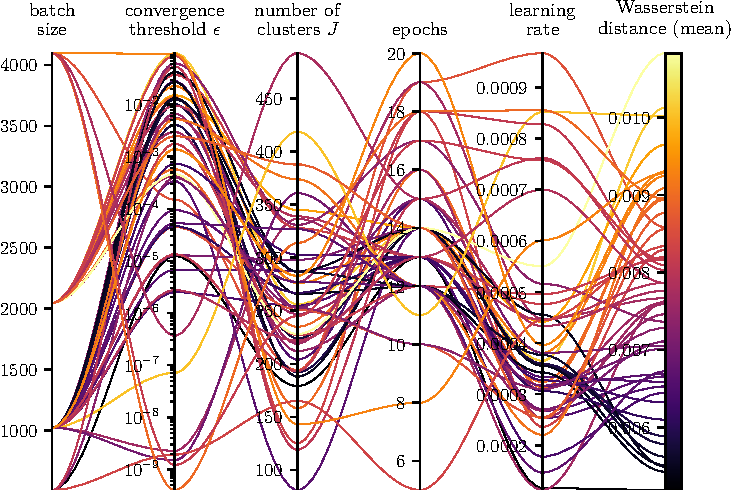
\includegraphics[scale=1]{content/plots/hyperparam/combined_pcplot_full.pdf}
  \caption{Parallel coordinates plot of the initial Bayesian hyperparameter search.}
  \label{fig:hyperparameter:bayesian}
\end{figure}

\begin{table}
    \centering
    \caption{
      Optimal hyperparameters as determined by a Bayesian optimization search.
    }
    \label{tab:hyperparameters:initial}
    \begin{tabular}{l S}
        \toprule
        Hyperparameter & {Value} \\
        \midrule
        %TODO: Placeholder values
        batch size & 512 \\
        learning rate & 0.0009 \\
        $J$-factor & 10 \\
        convergence threshold $\epsilon$ & 0.1 \\
        \bottomrule
    \end{tabular}
\end{table}


\subsection{Batch size}
The \emph{batch size} determines the number of events used for each training step.
While larger batch sizes increase the speed of training
on optimized hardware,
the performance of the model can be negatively affected \cite{batchsize_kandel}.
% NOTE: not-so-relevant citation

The boxplot in \autoref{fig:hyperparameter:batch_size} shows the results of a grid search for the batch size.
As expected, the performance is worse for larger batch sizes.
% TODO: Verify on an actual grid search (not just the Bayesian search results)

\begin{figure}
  \centering
  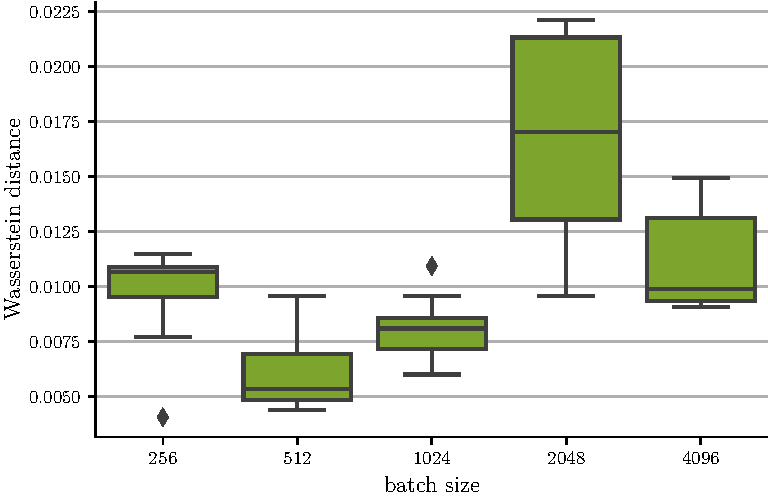
\includegraphics[scale=1]{content/plots/hyperparam/batch_size_vs_wd_boxplot_full.pdf}
  \caption{Boxplot of the performance of the model for different batch sizes.
    The performance is measured using the \emph{Wasserstein distance}.
    % TODO: Copilot | fact-check!
    % The whiskers extend to the 1st and 3rd quartile,
    % and outliers are shown as crosses.
  }
  \label{fig:hyperparameter:batch_size}
\end{figure}


\subsection{Convergence threshold}
% TODO: duplicate explanation?
When using adaptive step sizes,
instead of setting a fixed number of DSEA iterations,
a minimum $\Chi^2$ distance between iterations $\epsilon$
can be specified.
When the $\Chi^2$ distance becomes smaller than $\epsilon$,
convergence is assumed and the training is stopped.

\begin{figure}
  \centering
  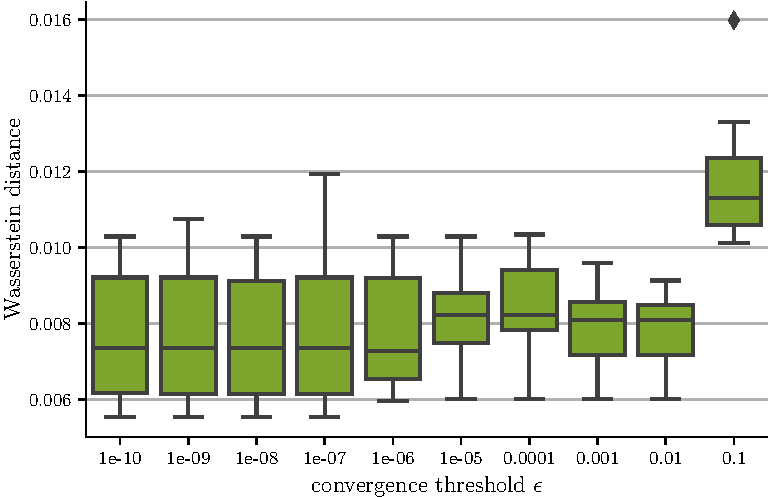
\includegraphics[width=0.75\textwidth]{content/plots/hyperparam/epsilon_vs_wd_boxplot_full.pdf}
  \caption{TODO.}
  \label{fig:hyperparameter:epsilon}
\end{figure}


\subsection{Adaptive step size: $J$-factor}
% TODO: Plot and explain J instead of J-factor?
The adaptive step size function,
  which has been explained in \autoref{sec:dsea:dsea:stepsize},
internally relies on clustering the data into $J$ clusters.
The number of clusters $J$ is therefore a hyperparameter of the algorithm.

Large values of $J$ have previously been shown to lead to slightly better results \cite{dsea_mirko}.

Because of the dependence of …,
$J$ is not used directly.
Instead, the \emph{J-factor} is used,
which is defined as $J$ divided by the number of bins.

\begin{figure}
  \centering
  % TODO: correct dimensions
  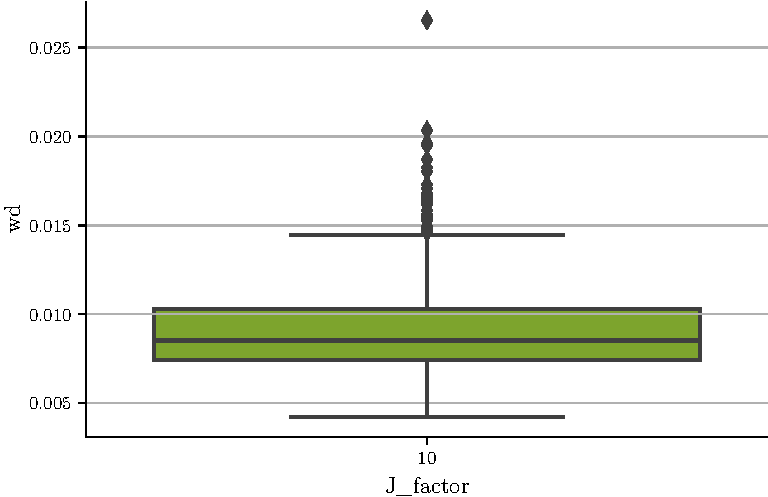
\includegraphics[scale=1]{content/plots/hyperparam/J_factor_vs_wd_boxplot_full.pdf}
  \caption{Boxplot of the Wasserstein distance for different $J$-factors.}
  \label{fig:hyperparameter:J_factor}
\end{figure}

\subsection{Number of epochs}
While a higher number of epochs typically increases the model's performance on the training data,
it also increases the risk of overfitting.



